\documentclass{beamer}
\usetheme{Boadilla}
\usecolortheme{whale}
\graphicspath{{../../figures/}}

\usepackage{wrapfig}

\title[MSc Thesis]
{Memristors-based Recurrent Modules for Neural Computing}
%\subtitle{Using }

\institute[IST] % (optional)
{%
  Diogo Caetano\\
  INESC-MN
  \and%
  Ruxandra Barlulescu\\
  INESC-ID
  }

  \author[V. BARBAZA]{Valentin BARBAZA (MEEC)}

  \date[2023] % (optional)
  {May 2023}

  \logo{
\includegraphics[height=0.7cm]{logos/ist}}

  \definecolor{istblue}{RGB}{0,102,153}
  \setbeamercolor{titlelike}{bg=istblue}
  \setbeamerfont{title}{series=\bfseries}

  \begin{document}

  \frame{\titlepage}

  %\begin{frame}
  %\frametitle{Table of Contents}
  %\tableofcontents
  %\end{frame}

  \begin{frame}
    \frametitle{Application/Motivation}
    The goal of the thesis is to know whether an analog LSTM network would work. This would allow running a Neural Network in real-time in embedded systems. The analog implementation (using memristors crossbar array) allows for much greater computational speed and very small on-chip area.
  \end{frame}
  \begin{frame}
    \frametitle{Technical Goals}
    My point is to run simulations using cadence. Running a working simulation is the first step before fabricating the system.
  \end{frame}
  \begin{frame}
    \frametitle{Progress}
    So far, I have designed some smaller elements required for the system to work such as the activation function for example.\\
    I've designed a full size LSTM (with 4 hidden state).
    \begin{figure}
      \centering
      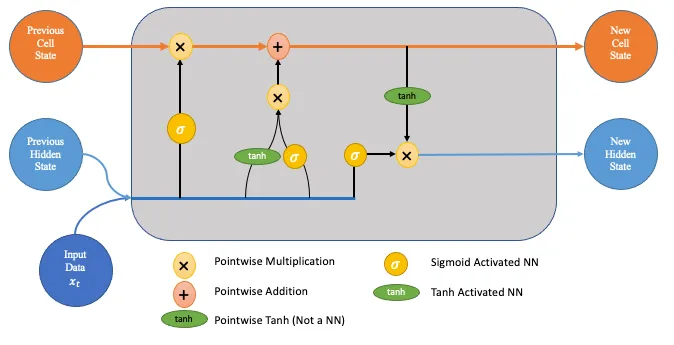
\includegraphics[height=0.35\textheight]{lstm/lstm.png}
    \end{figure}
    I am now working on a way to generate LSTM network of any size.
  \end{frame}

  \begin{frame}
    \frametitle{What is missing}
    I now need to run the simulations and compare the results of my simulation with the results a digital LSTM (running with Keras for example).
  \end{frame}

  \end{document}
